\documentclass{article}
\usepackage{graphicx}

\begin{document}

\section{Regression Test of GVTK}
Date: 05/02/2023 17:35:56

\vspace{5pt}

\noindent Regression Test Status: PASSED

\vspace{5pt}

\noindent This test case is completed using 6 particles from the Cylindrical Flow dataset. Passing of this test means no changes in results have occurred with the new additions made to the toolkit.
The standard edition of GVTK used for this testing is the November 2022 release. If you are wanting to complete changes in the physics that results in differences in final velocity and the forces,
you will fail this test. Please update the rest of the team if this is the case before moving on. This test will give you a summed error across the timesteps for all forcing terms to see which terms
are changing most drastically due to the updates to help guide debugging or physics updates. FAILURE WILL RETURN A DIVIDE BY ZERO ERROR TO PREVENT MERGERS!



\vspace{5pt}

\noindent Summary of Summed Errors:
\vspace{5pt}

Velocity Error: 0.0

Position Error: 0.0

Drag Error: 0.0

ShearGradLift Error: 0.0

Body Force Error: 0.0

\vspace{5pt}

\noindent Summary/Actions: No action needed, regression test passed and it is safe to push new version to GitLab

\vspace{5pt}

\noindent Please report any differences. If making updates that are non-physics based, this test MUST BE PASSED before any commits to gitlab!

\begin{figure}[htbp]
\centering
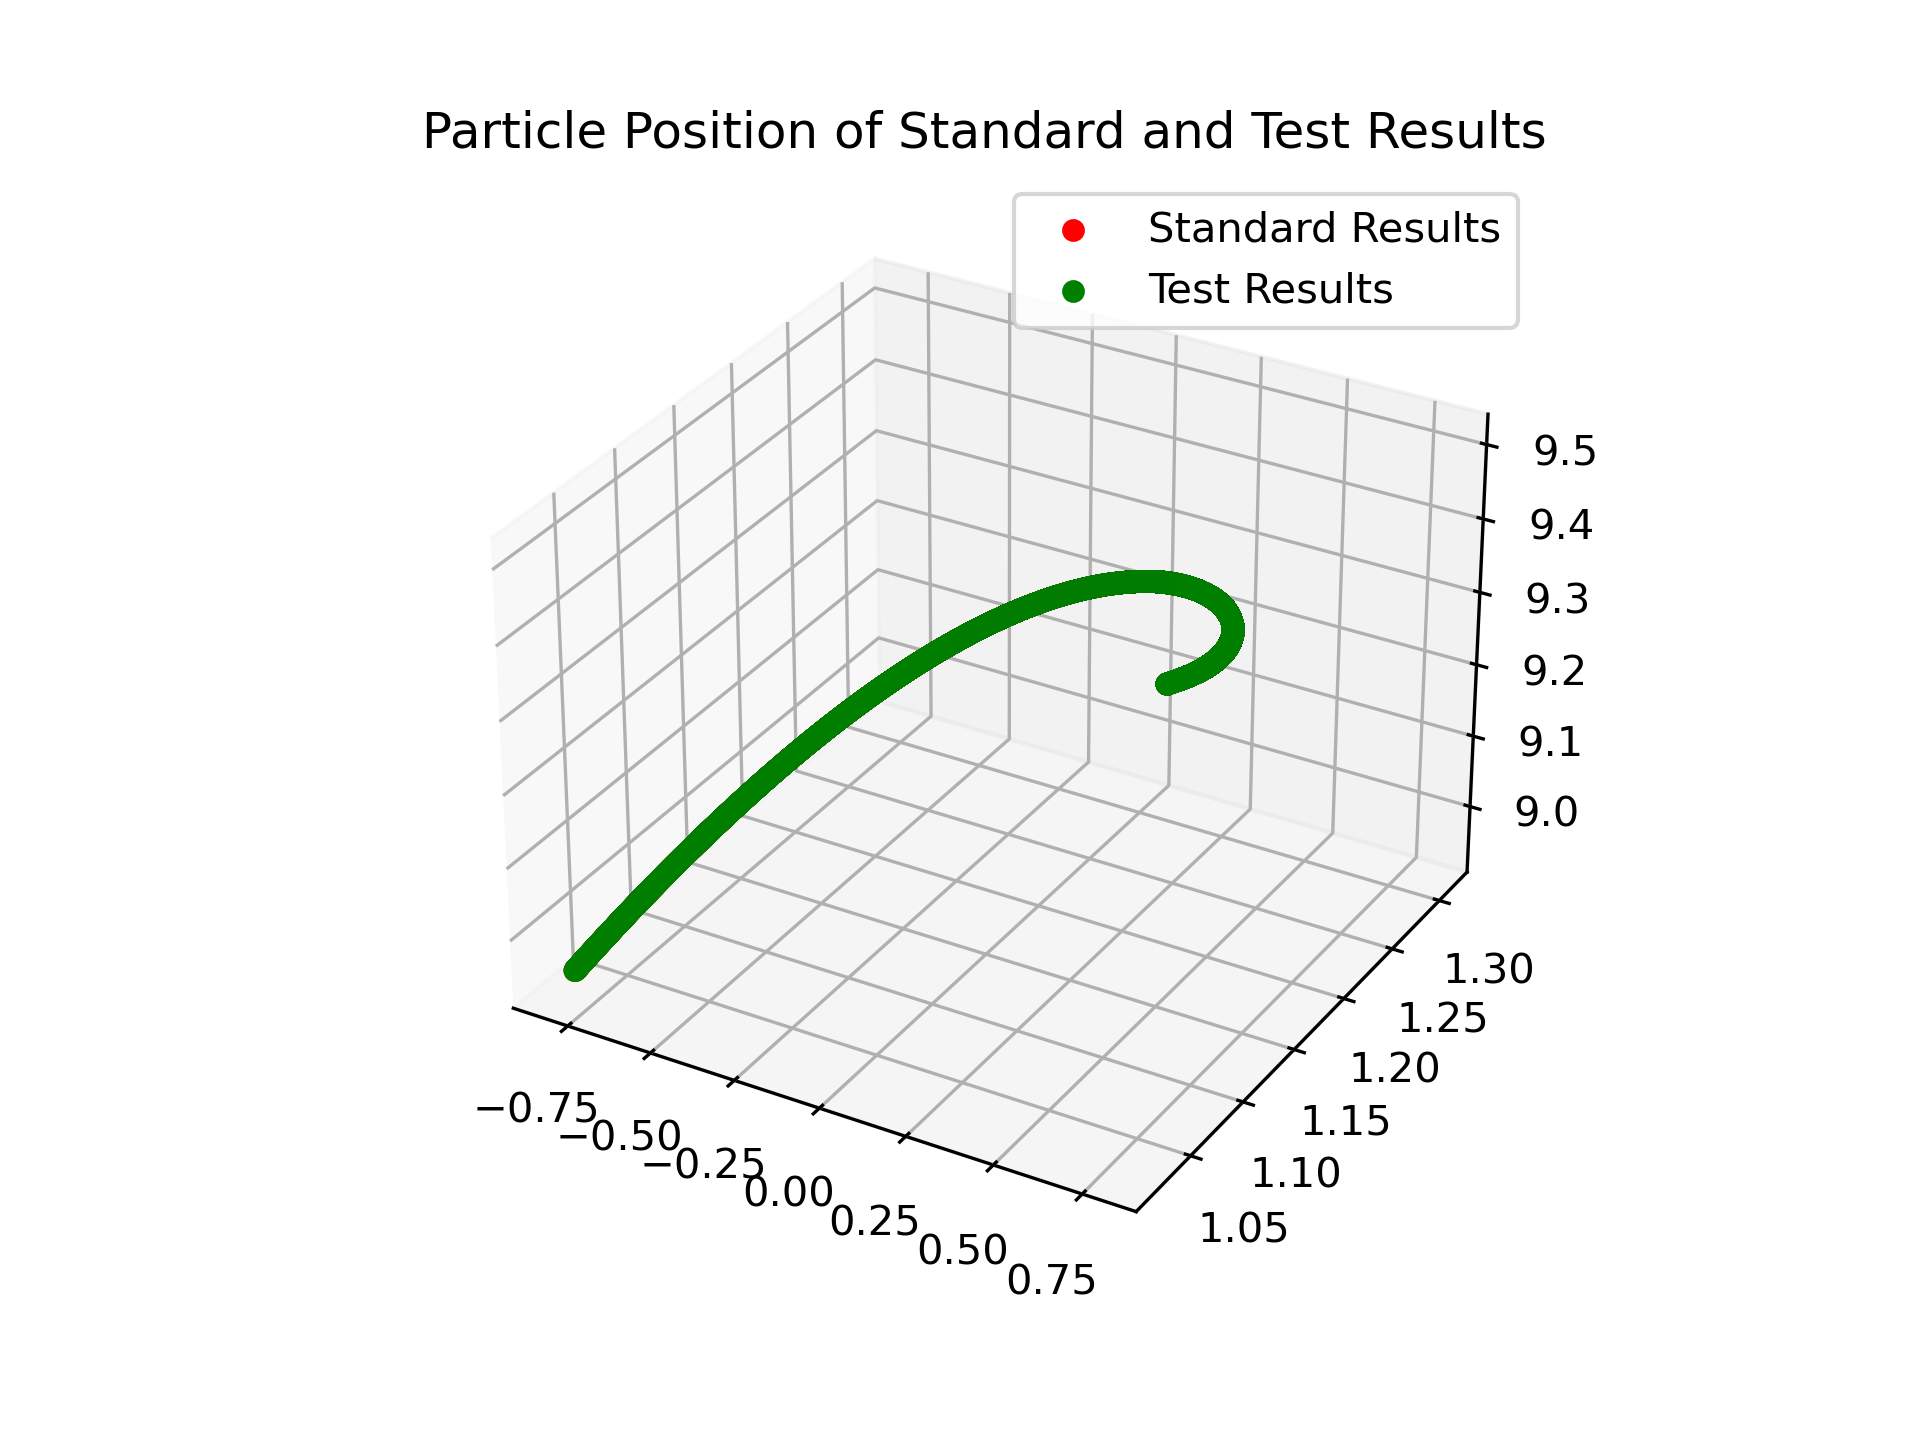
\includegraphics[width=1.0\textwidth]{Position.png}
\caption{\textit{Position of the particle for both the test and standard results}}
\label{fig:postion}
\end{figure}

\end{document}
